% !TeX encoding = UTF-8
% !TeX program  = xelatex

\documentclass[12pt,a4paper]{article} 
\usepackage[typeblock=wide]{stb-titlepage}        

%==== Math setup =====================================================
\usepackage{amsmath}%............................. Advanced math (before fonts)
%\usepackage{amssymb}%............................ AMS Symbol fonts

%==== Font setup =====================================================
\usepackage{iftex}
\ifxetex
    \usepackage[math-style=TeX,
                bold-style=TeX,
               ]{unicode-math}
    \setmainfont{Cambria}%........................ Unicode fonts  (Win)                
    \setsansfont[Scale=MatchLowercase]{Calibri}
    \setmonofont[Scale=MatchLowercase]{Consolas}
    \setmathfont{Cambria Math}
    \defaultfontfeatures{Ligatures=TeX}
    \let\bm\symbfit
\else
    \usepackage[utf8]{inputenc}%.................. Unicode file format
    \usepackage{textcomp}%........................ Additional text symbols
    \usepackage[T1]{fontenc}%..................... Type 1 outline fonts
    \usepackage{bm}%.............................. Bold math fonts
\fi
\normalfont

%==== Units and numbers ==============================================
\usepackage{siunitx}%............................. Unit, number and angle output
    \sisetup{detect-all = true, detect-family = true}
    \sisetup{output-decimal-marker = {.} ,
             group-separator = {\,},
             number-unit-product = {\,},
             inter-unit-product = \mathord{\cdot},
             exponent-product = \mathord{\times},
             separate-uncertainty = true}
         
%==== Ref's, Bib's and Nomencl =======================================
\usepackage{stb-nomencl}%......................... List of symbols 
    \renewcommand*{\UnitLabel}[1]{~[\,\unit{#1}\,]}
\usepackage{stb-bib}%............................. Bibliography (natbib internally)
    \bibliographystyle{stb-bib-eng-a}
    \renewcommand\bibfont{\small}

%==== Tables + Graphics + Color =====================================
\usepackage{array}%............................... Extended table defs 
    \setlength{\extrarowheight}{2pt}
\usepackage{booktabs}
   \heavyrulewidth=\lightrulewidth
   \cmidrulewidth=\lightrulewidth
   \abovetopsep=\smallskipamount
   \belowbottomsep=\smallskipamount
   \cmidrulekern=\tabcolsep
\usepackage{graphicx}%............................ Included graphics
\usepackage[font=small]{caption}%................. Customize captions  
\usepackage[table]{xcolor}%....................... Color setup + colortbl 

%==== User Defs ======================================================
\makeatletter
%
% Please insert user defined commands here
% and NOT in the document itself!
%
%
\newcommand\f{\mathfrak{f}}          % Friction factor
\newcommand\vf{\bar{\varepsilon}}    % Bed void ratio

\newcommand\usubi[2]{_{{\mathrm{#1}}{#2}}}
\newcommand\bed[1][]{\usubi{b}{#1}}  % Packed bed
\newcommand\elm[1][]{\usubi{p}{#1}}  % Packed bed element
\newcommand\hs[1][]{\usubi{r}{#1}}   % Rock Heat store

\makeatother

%==== Title Page =====================================================
\title{{\large System Simulation Notes}\\
       \textbf{Rock Bed Heat Storage}}                   
\author{Danie Els}                
\address{Department of Mechanical and Mechatronic Engineering\\
        Stellenbosch University \\
        Private Bag X1, Matieland 7602}
\date{2023/01/05}                             
\Copyright{2023}{Stellenbosch University.\\ All rights reserved.}

\begin{document}
\maketitle 
\begin{abstract}
A rock bed is modeled as a porous medium ...
\end{abstract}

\section*{List of symbols}
\begin{Nomencl}[1.0em]
\NomGroup{Variables}
    \item[$a$]        \UnitLine{surface area           }{m^2}
    \item[$A$]        \UnitLine{area                   }{m^2}
    \item[$c_{p}$]    \UnitLine{specific heat capacity }{J/(kg.K)}
    \item[$\dot{m}$]  \UnitLine{air mass flow rate     }{kg/s}
\end{Nomencl}

\begin{figure}[htbp]
    \centering
    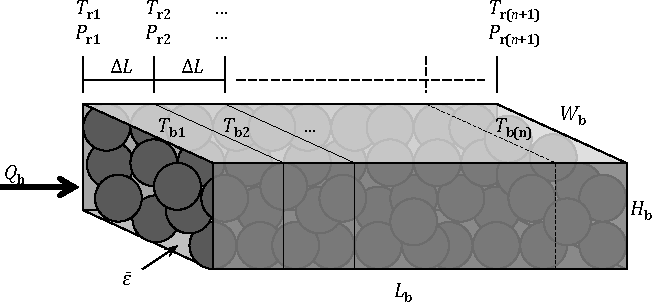
\includegraphics[scale=1]{figs/bed}
     \caption{Packed bed heat store}
    \label{fig:Bed}
\end{figure}

\section{Packed bed material properties}

Consider the packed bed heat store shown in figure~\ref{fig:Bed}. It is filled with
spherical stones. Define the average \emph{void fraction} $\vf$ as
\begin{equation}
    \vf = \frac{\text{volume of empty space}}
               {\text{volume of solid media}}
\end{equation}

Assume that the flow is uniform and one-dimensional through the bed. The projected
flow area $A\bed$ perpendicular to the flow direction is
\begin{equation}
    A\bed = W\bed\,H\bed
\end{equation}
with $W\bed$ and $H\bed$ the bed width and height.

The different fractions of solids and air are given in table~\ref{tab:bed-prop}. 
\Citet{Beasley-1984} give the average void fraction as a function of container diameter to particle diameter for uniform spheres. 

\begin{table}[htbp]
    \centering
    \caption{Fractions of air and solids in packed bed}
    \label{tab:bed-prop}
    \begin{tabular}{@{}lll@{}}
        \toprule
                 & \multicolumn{1}{c}{Air}     & \multicolumn{1}{c}{Solids}      \\
        \cmidrule(lr){2-2}\cmidrule(l){3-3}
        Fraction & $\vf$                       & $(1-\vf)$                        \\
        Volume   & $\vf\, A\bed\, L\bed$           & $(1-\vf)\, A\bed\, L\bed$            \\
        Mass     & $\vf\, A\bed\, L\bed\,\rho\hs$ & $(1-\vf)\, A\bed\, L\bed\, \rho\elm$ \\
        \bottomrule
    \end{tabular}
\end{table}


\section{Heat transfer between the bed and the air}

\section{Temperature change in the bed}

\section{Calculation procedure}


\bibliography{packed-bed.bib}

\end{document}
